\documentclass{report}
\usepackage[english]{babel}
\usepackage[utf8]{inputenc}
\usepackage[T1]{fontenc}
\usepackage{listings}
\usepackage{titlesec}
\usepackage{color}
\usepackage{graphicx}

\titleformat{\chapter}[display]
            {\normalfont\bfseries}{}{0pt}{\Huge}

\lstset{ escapeinside={(*}{*)} }

\title{Rapport IA PROG6}
\author{Castel Antonin}
\begin{document}
\maketitle{}

\chapter{Introduction}
Le jeu Pingouin est un jeu à somme nulle où un certain nombre de joueurs s'affrontent à tour de rôles. Une IA difficile peut donc utiliser un algorithme de type MinMax pour évaluer les coups possibles.Pour créer l'IA la plus efficace possible, nous avons identifié trois grandes phases de jeu lors du déroulement de chaque parties :
\newline

-Le placement des pingouins en début de partie sur les cases à un poisson.


-Les déplacements en début de partie, lorsque l'algorithme MinMax ne calcule 
pas assez de coups à l'avance pour différencier avec pertinence les différents coups possibles.


-La fin de partie, où les quelques coups d'avance que calcule le MinMax sont 
suffisant pour évaluer la qualité d'un coup.

Nous allons donc détailler ici comment son gérés ces différentes phases dans notre IA difficile, et comment sont utilisés des parties de l'IA difficile pour créer des IA plus simple.
\chapter{IA Difficile}
Notre IA difficile à une stratégie bien définie, à la fois maximiser le nombre de poissons récupérés et faire des îles, soit pour enfermer les pingouins ennemis, soit pour s'assurer une grande quantité de poissons en fin de partie.
Pour ce faire, nous avons utilisé un algorithme de type MinMax avec élagage Alpha-Beta.
\section{Placement en debut de partie}
En début de partie, il n'est possible de se placer que sur des cases contenant un seul poisson, nous calculons donc une heuristique sur chaque case contenant un poisson, et notre pingouin est placé sur la case ayant la meilleure heuristique.
Ces heuristiques sont calculées pour chaque cases en fonction du nombre de cases a trois poissons voisines accessibles. 
\newline
On prend aussi en compte le fait que placer un pingouin sur un bord de la carte n'est pas une bonne idée (encore moins dans un coin), ainsi que du fait qu'il faut éviter de mettre tout ses pingouins dans la même zone de la carte.
\newline
On prend aussi en compte le placement des pingouins ennemis, car on tente de les priver du plus grand nombre de cases possible.


\section{Structures de données et fonctionnement du MinMax}
Nous avons un structure Plateau, contenant le plateau de jeu et différentes méthodes qui permettent entre autres de jouer un coup donné et de revenir en arrière sur le dernier coup exécuté.
\newline
Nous les utilisons donc pour simuler les coups sur le plateau de jeu initial, sans cloner le plateau ni stocker l'arbre.



\section{Heuristiques}
Nous avons deux calculs d'heuristiques distincts, l'un pour évaluer les feuilles de l'arbre (et donc un ensemble de coup joué sur le plateau de jeu initial), et un autre pour évaluer les coups possible directement sur la configuration de base.
\newline 
Cela signifie que lorsque les heuristiques sont calculés sur les feuilles et qu'elles remontent à la racine, elle sont re-évalués en fonction du coup qui sera joué directement par l'IA.
\newline
La raison pour cette re-évaluation des heuristiques est double :

\hspace{0.5cm}	-D'une part, cela permet de départager les fils de la racine qui ont une heuristique identique, c'est donc très bien en début de partie, ou MinMax ne calcule pas une profondeur assez grande pour que les heuristiques soient pertinentes. \newline
Si deux fils de la racine (donc deux coups possibles) ont la même heuristiques calculée par le MinMax, il vaut mieux choisir celui dont le coup est le plus avantageux.

\hspace{0.5cm}	-D'autre part, cela permet à l'IA de ne pas faire de coups mauvais, car comme on calcule les heuristiques aux feuilles, on évalue un ensemble de coups dans sa globalité, par conséquent il est possible qu'un configuration soit considérée comme favorable par le MinMax alors qu'un coup très mauvais fait partie de l'ensemble de coups permettant d'aboutir à cette configuration (par exemple ça évite d'isoler un pingouin allié, ce qui est toujours une mauvaise idée).

\vspace{0.7cm}
La re-évaluation est de moins en moins importante lorsqu'on avance dans la partie, ce qui signifie qu'on fait de plus en plus confiance aux résultats du MinMax, jusqu'à un point où la re-évaluation est dérisoire par rapport aux heuristiques des feuilles.
\newline
Cela represente donc bien les deux grandes phases de jeu :
\newline
-Celle où la re-évaluation des heuristiques est utile pour choisir le meilleur coup.
-Celle où les heuristiques calculés par le MinMax sont les plus importantes.
\newpage
\textbf{Heuristiques calculées sur les feuilles :}
\newline
Les heuristiques sur les feuilles sont calculés en fonction des îles présentes sur le plateau de jeu, et sur les scores des différents joueurs.
\newline
On calcule la liste des îles, et on évalue chacune d'entre elles en fonction du nombre de poissons qu'elle contient ainsi que du nombre de pingouins alliés et du nombre de pingouins ennemis qu'elle contient.
\newline
Par exemple, laisser une île à l'ennemi n'est pas une bonne idée, sauf si tout les pingouins ennemis sont sur cette île et que cette dernière n'a pas suffisamment de poissons pour que l'ennemi puisse gagner.
\newline 
La configuration est donc évaluée en fonction de ses îles et de ce qu'elles contiennent.
\newline 
En particulier,
\newline
-On essaie de ne pas laisser de trop grandes parties de banquise à un pingouin ennemi seul.
\newline
-On essai de s'isoler sur une grande partie de banquise. 
\newline
-On évite de laisser des grandes îles sans aucun pingouins dessus. 
\newline
-Si la partie est finie et que notre score est le plus élevé, on renvoie une heuristique maximale.
\newline
-Si un ou plusieurs pingouins ennemis sont isolés sur une île suffisamment grande pour s'assurer la victoire, on renvoie une heuristique minimale.

\vspace{0.3cm}
\textbf{Heuristiques calculées sur les fils de la racine :}
\newline
Ces heuristiques n'ont pas le même but, elles sont calculé en fonction d'un seul coup, et donc on vérifie que l'IA ne va pas isoler un de ses pingouins, qu'elle ne passe pas à coté de l'opportunité d'isoler un pingouin ennemi ou qu'elle ne condamne pas un autre de ses pingouins en faisant ce déplacement (sans l'isoler directement).
\newline
On favorise aussi le fait de bloquer l'adversaire, on tente de se placer sur une case accessible par le plus de pingouins ennemis possible, en essayant de leur bloquer l'accès au plus grand nombre de cases possible.
\vspace{0.3cm}

\section{Fin de partie}
Durant toute la durée de la partie, un pingouin isolé sur son île n'est pas considéré par le MinMax, et ne sera donc jamais déplacé.
C'est donc à la fin de la partie que l'on doit calculer le meilleur chemin sur une île, pour chaque pingouin.
\newline 
Pour ce faire, on calcule un parcours Eulérien sur l'île. La complexité pour trouver un parcours Eulérien est telle que malheureusement sur une grande île, on ne peut pas le calculer. Quand c'est le cas, on fait un coup pseudo-aléatoire (on essaye de ne pas casser le parcours Eulérien, sans le calculer) jusqu'à que la taille de l'île soit suffisamment petite pour qu'on puisse faire le parcours.

\chapter{IA facile et IA moyenne}

\section{IA moyenne}
L'IA moyenne est basée sur l'IA difficile, sauf qu'elle calcule une partie de l'arbre bien inférieure à l'IA difficile, et par conséquent ses coups sont moins réfléchis.
Pour l'IA moyenne, le calcul heuristique des fils de la racine est aussi important que celui des feuilles.
\section{IA facile}
L'IA facile se comporte comme l'IA difficile pour la première phase de jeu, mais sa stratégie est très différente, elle n'est pas aléatoire mais essaie de récupérer le plus de poisson possible en le minimum de coups, elle récupère donc rapidement beaucoup de points, mais elle ne priorise pas forcement le fait de bloquer un ennemi.
Cela donne une IA qui n'est pas très performante quand il y a peu de pingouins pour beaucoup de cases, mais une IA très correcte lorsque la tendance s'inverse.


\chapter{Changements possibles}
\section{Améliorations possibles des IA}

-L'IA difficile ne change pas de stratégie quand la sienne n'est pas la bonne. Il a été dit plus haut que la stratégie de l'IA facile était très correcte quand le nombre de pingouins est très grand comparé au nombre de cases, par conséquent, l'IA difficile pourrait changer de stratégie dans ce genre de cas.
\newline
-Le parcours Eulérien en fin de partie sur les grandes îles est largement améliorable.
\newline 
-On pourrait Multithreader le calcul de l'arbre pour améliorer significativement la profondeur calculable de ce dernier, et donc largement améliorer le niveau de jeu de l'IA.

\section{Pistes explorées mais non concluantes}
-On pourrait utiliser MinMax pour calculer le parcours Eulérien en fin de partie, comme il essaie de maximiser le score, on obtiendrait un chemin très correct.
\newline
-Nous avons essayé de modifier la profondeur de calcul de l'arbre localement, pour que les branches prometteuses soit calculées plus profondément que les branches où les premiers coups sont mauvais, mais les résultats n’étaient pas très concluants en terme de niveau de jeu de l'IA.











\chapter{Résultats}

\begin{center}
  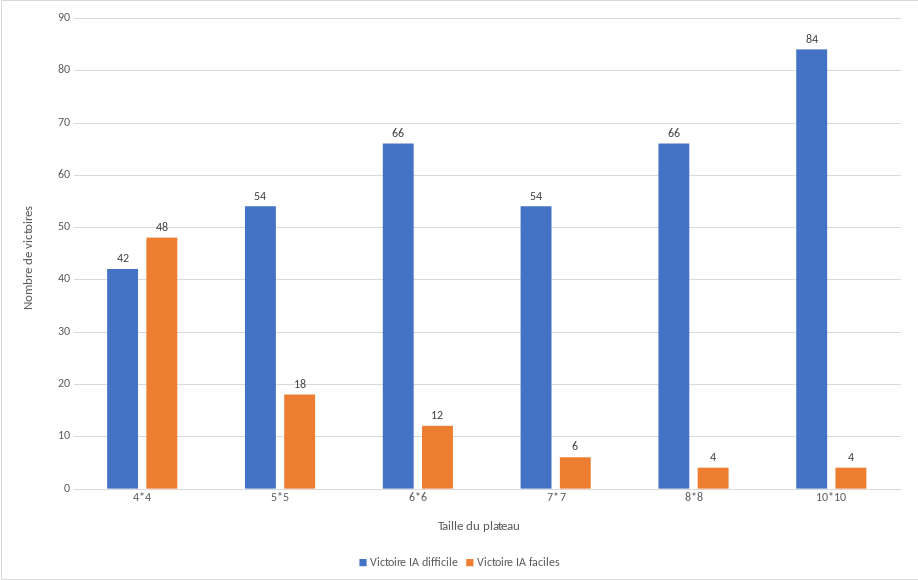
\includegraphics[width=9cm]{graph1.png}
\end{center} 
\textbf{\textit{Difficile vs facile sur différents plateaux.}}
\begin{center}
  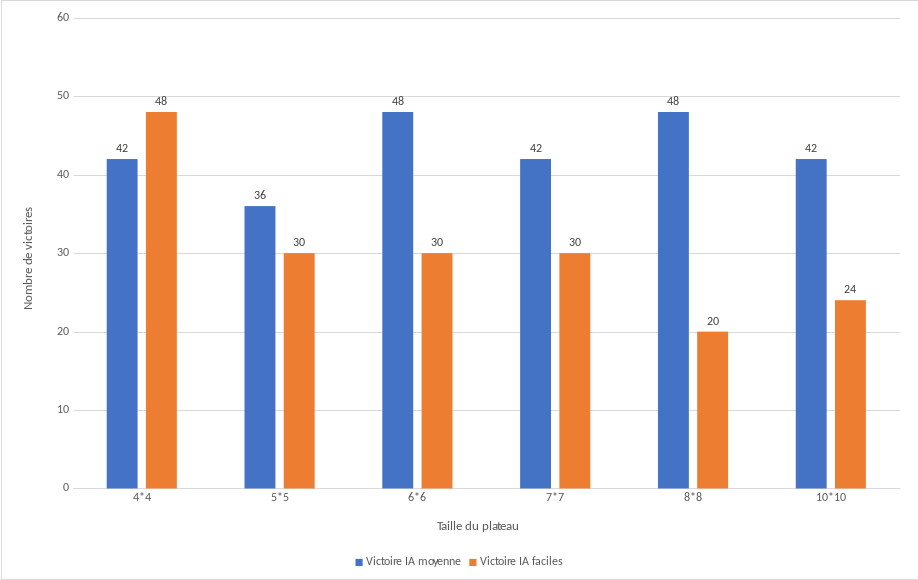
\includegraphics[width=9cm]{graph2.png}
\end{center}
\textbf{\textit{Moyenne vs facile sur différents plateaux.}}
\chapter{Conclusion}

Nous pouvons voir que les IA respectent assez bien la hiérarchie difficile > moyenne > facile entre elles. 
Les parties représentées dans ces graphiques représentent des parties à deux joueurs avec 4 pingouins, les tendances sont exactement les mêmes si on modifie le nombre de pingouins par joueurs.
Cette hiérarchie est aussi assez bien respectée lors des parties avec un nombre de joueurs supérieur à deux, mais vu que nous nous sommes concentrés en priorité sur les parties à deux joueurs, il existe des anomalies que nous n'avons pas eu le temps de résoudre.
\newline
Par exemple, une partie à quatre joueurs, avec 3 IA difficiles et une IA facile sur un plateau de taille standard sera souvent remportée par l'IA facile, simplement car sa stratégie est bien supérieure à celles des IA difficiles dans cette situation.
\newline
Contre les humains, un graphique du même genre serait malheureusement assez trompeur. En effet, l'IA difficile gagne rarement, mais sans que ce soit une victoire écrasante pour le joueur. Les scores finaux sont généralement très proche l'un de l'autre.


\end{document}